% #region PREAMBEL OG PAKKER
\documentclass[a4paper, 12pt]{article}  % DOKUMENTKLASSE
\title{Øving 9}                         % TITTEL
\author{Håvard Solberg Nybøe}           % FORFATTER
\date{MA0301}                           % DATO & FAG

\usepackage[english, norsk]{babel}      % NORSK SPRÅK
\usepackage[
    backend=biber,style=apa]{biblatex}  % BIBLIOGRAFI
\usepackage{csquotes}                   % PAKKE TIL BABEL
\addbibresource{bibliografi.bib}         % PATH TIL BIBLIOGRAFI
\usepackage[hidelinks]{hyperref}        % LENKER I TOC OG GENERELT
\usepackage[margin=1in]{geometry}       % VANLIG STØRRELSE MARGIN
\setlength{\parindent}{0em}             % SKILLER AVSNITT
\setlength{\parskip}{.8em}              % SKILLER AVSNITT
\usepackage{graphicx}                   % BILDER \includegraphics[OPTIONS]{PATH}
\usepackage{kantlipsum}                 % FYLLTEKST I KANT-STIL (kant[n-m])
\usepackage{amsfonts,                   % BLACKBOARD BOLD FONT (\mathbb{N})
amsmath,stmaryrd,amssymb}               % ANDRE MATTE PAKKER
\usepackage{circuitikz}                 % LOGISKE PORTER OG KRETSER & TikZ
\usepackage{import}                     % IMPORTER FILER (\import{PATH}{FILE})
\usepackage{caption}                    % PAKKE FOR BEDRE CAPTIONS I FIGURER
\usepackage{float}                       % FLYTT FIGURER 
% #endregion
\begin{document}

\maketitle
% \tableofcontents % INNHOLDSFORTEGNELSE

\begin{enumerate}
    \item [\boxed{1}]
    \begin{enumerate}
        \item 
        \begin{equation*}
            \left[
                \begin{array}{ccccc}
                    1 & 1 & 0 & 0 & 0 \\
                    0 & 1 & 1 & 0 & 1 \\
                    0 & 0 & 0 & 1 & 1 \\
                    1 & 0 & 1 & 1 & 0 \\
                    0 & 0 & 0 & 0 & 0
                \end{array}
            \right]
        \end{equation*}
        \begin{figure}[h!]
            \centering
            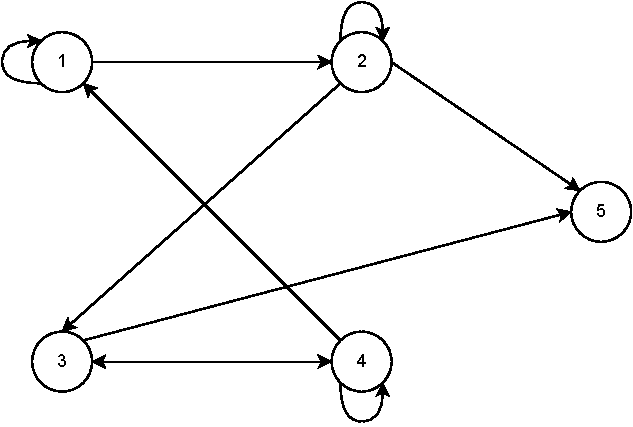
\includegraphics{graf1.pdf}
        \end{figure}
        \newpage
        \item 
        \begin{equation*}
            \left[
                \begin{array}{ccccc}
                    0 & 1 & 1 & 0 & 1 \\
                    1 & 0 & 0 & 1 & 1 \\
                    1 & 0 & 0 & 0 & 0 \\
                    0 & 1 & 0 & 0 & 1 \\
                    1 & 1 & 0 & 1 & 0
                \end{array}
            \right]
        \end{equation*}
        \begin{figure}[h!]
            \centering
            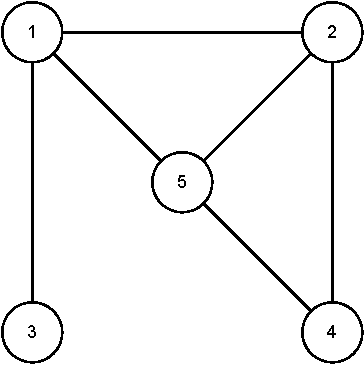
\includegraphics{graf2.pdf}
        \end{figure}
    \end{enumerate}
    \item [\boxed{2}]
    \begin{enumerate}
        \item Grafen må ha en euler vei fordi graden til hjørene i grafen er et partall. 
        \\ \(B-A-G-F-E-D-C-E-A-C-F-B\) er en euler vei i grafen.
        \item Hvis hjørnene \(e \text{ og } f\) fjernes fra grafen vil ikke grafen være sluttet sammen eller ha en euler vei.
        \item Hvis hjørnene \(e, f, g\) fjernes fra grafen, vil ikke grafen være sluttet sammen eller ha en euler krets.
    \end{enumerate}
    \item [\boxed{3}] \text{}
    \begin{figure}[h!]
        \centering
        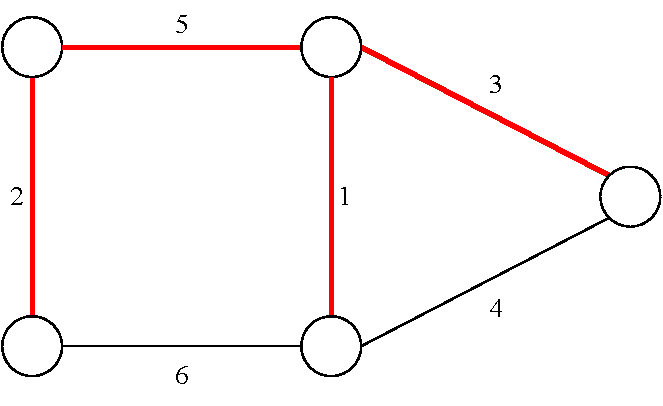
\includegraphics{graf3.pdf}
    \end{figure}
    \newpage
    \item [\boxed{4}]
    \begin{enumerate}
        \item \text{}
        \begin{figure}[h!]
            \centering
            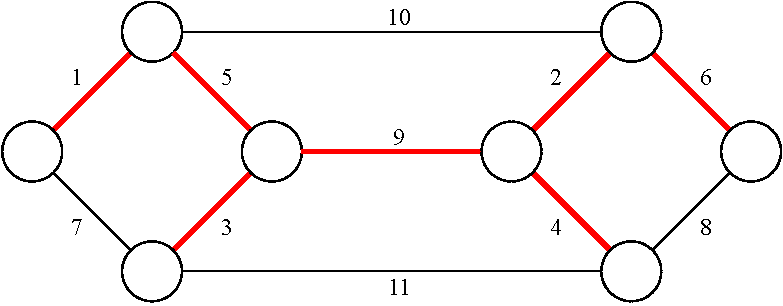
\includegraphics{graf4.pdf}
        \end{figure}
        \item \text{}
        \begin{figure}[h!]
            \centering
            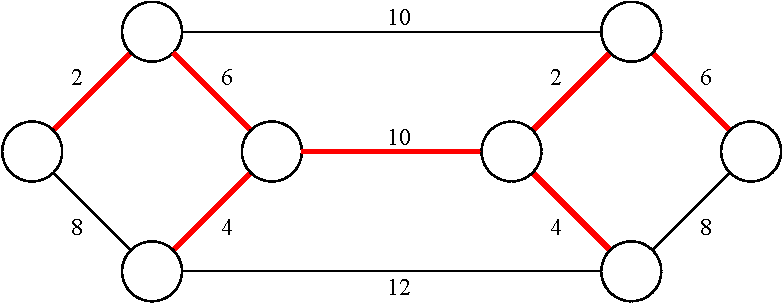
\includegraphics{graf5.pdf}
            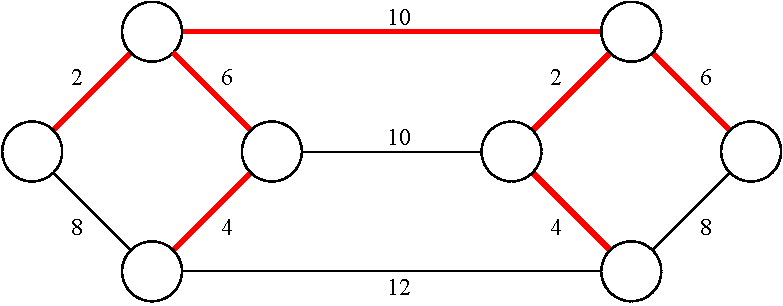
\includegraphics{graf6.pdf}
        \end{figure}
    \end{enumerate}
    \item [\boxed{5}] La \(G = (V, E)\) være en graf.
    \\ Anta at det finnes to forskjellige minste utspringstrær \(T_1 = (V, E_1)\) og \(T_2 = (V, E_2)\).
    \\ Siden \(T_1\) og \(T_2\) er forskjellige, er mengdene \(E_1 - E_2\) og \(E_2 - E_1\) ikke tomme mengder, altså \(\exists e \in E_1 - E_2\).
    \\ Siden \(e \in E_2\), vil å legge den til i \(T_2\) lage en sykel. Syklens har egenskapen at en mest vektede kanten, \(e'\), 
    ikke er i noen av de minste utspringstrærene. Men
    \\ Hvis \(e' = e\)
    \\ Så vil \(e' \in E_1\), fordi \(e \in E_1 - E_2\)
    \\ Hvis \(e' \neq e\), så vil \(e' \in E_2\)
    \\ Begge påstandende er motsigende med at \(e'\) ikke er i noen av de minste utspringstrærene. \(\square\)
    \item [\boxed{6}] Bruker en liknende modifisert graf fra forrige oppgave.
    \begin{figure}[h!]
        \centering
        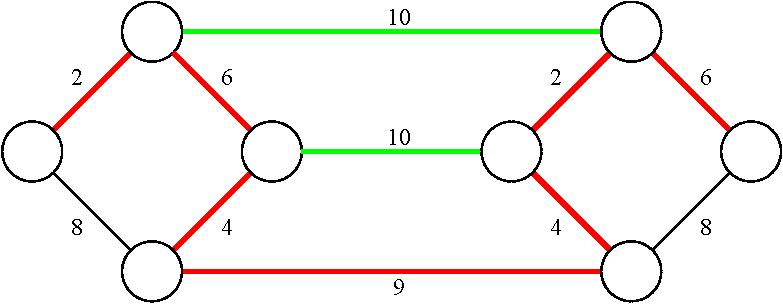
\includegraphics{graf7.pdf}
    \end{figure}
    \\Den røde stien er det minste utspringstreet, med en samlet vekt \(33\). Man kan bytte ut kanten med vekt \(9\) men en av de med vekt \(10\) og få to ulike utspringstrær hvor begge har en samlet vekt på \(34\).
\end{enumerate}

% \printbibliography[heading=bibintoc] % LAGER BIBLIOGRAFI
\end{document}
